\chapter{Front end implementation : Building a working UI}

\section{User's Manual}

\begin{figure}[h!]
\centering
\includegraphics[width=0.75\textwidth]{C5/project_workflow.png}
\caption{The iterative learning workflow}
\end{figure}
\mbox{}\\
This tool implements an iterate approach to learning. Start by entering some examples that may synthesise your desired output. Then, examine the returned Haskell and iteratively add more examples, fix incorrect ones and re-learn until you are happy with the result.

\subsection{Entering examples}

In order to use this tool, you first have to enter examples to learn, which specify how the target program behaves on specific inputs.\\ \\
You can change the number of input arguments by editing the "No. Args" box. While there are no restrictions on the possible arguments, be aware that any increase in number of arguments can greatly affect learning performance. Currently, the only supported argument type is Integer. 

\begin{figure}[h!]
\centering
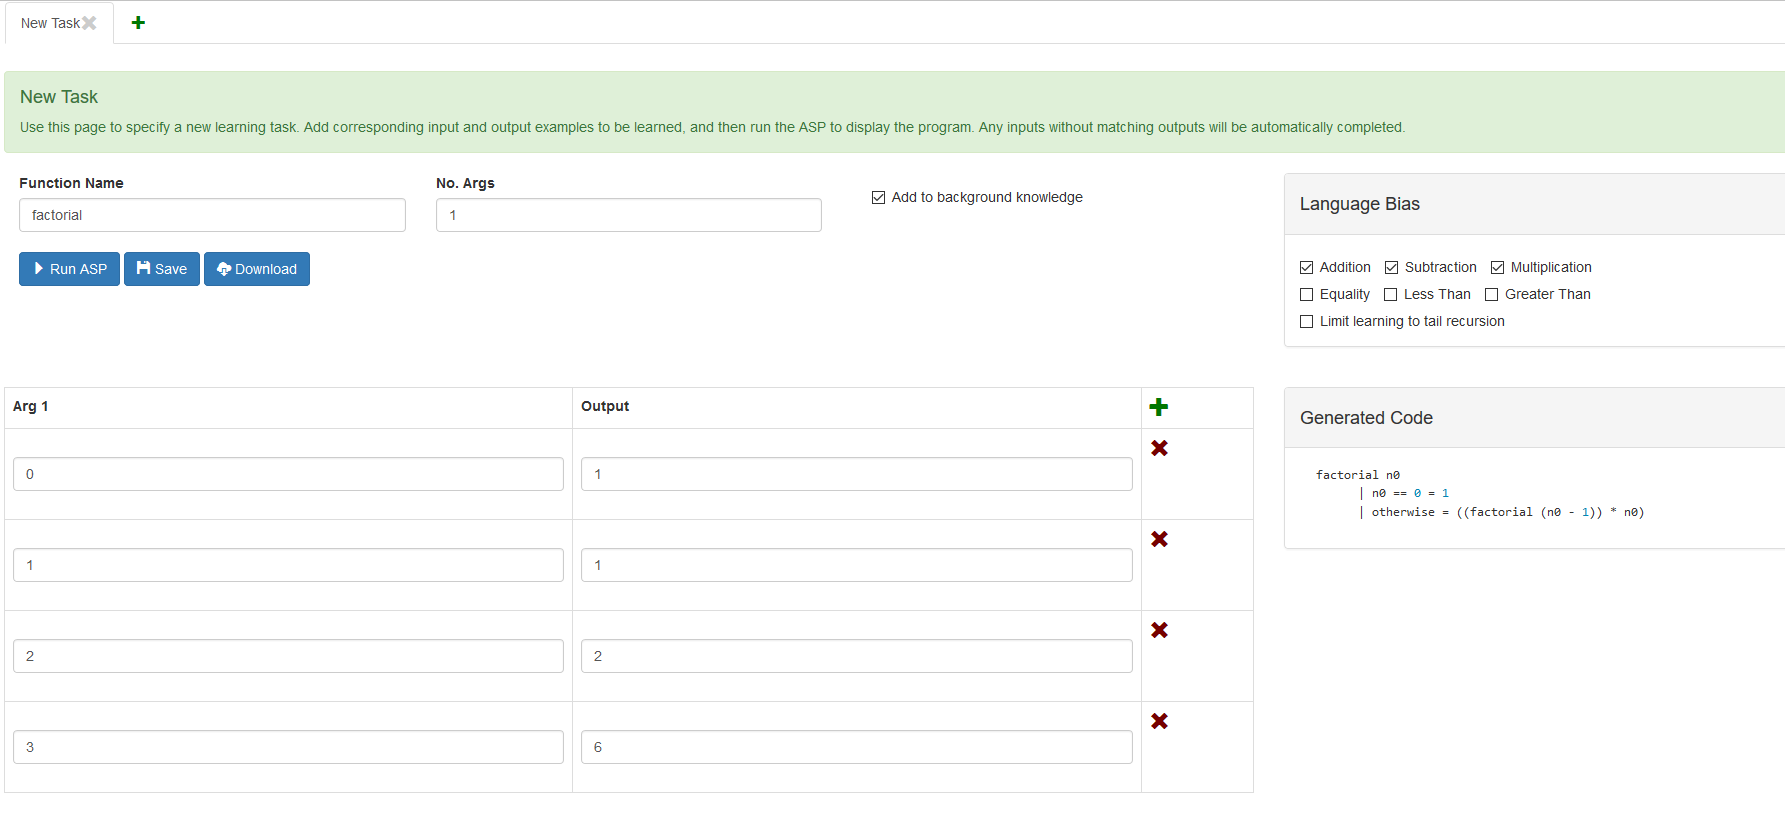
\includegraphics[width=\textwidth]{C5/screenshot_completed.png}
\caption{Learning Factorial}
\end{figure}

\subsection{The Learning Step}

After entering your examples, you can perform learning by clicking the "Run ASP" button. \\ \\
After a short computation step, the learned haskell is displayed, and there are a few options on how to proceed : 

\begin{itemize}
\item If the learned program is incorrect, then you can freely add more examples which specify the missing behaviour.
\item If you are unsure about the correctness of the program, you can simply test some more complicated answers using example autocompletion.
\item If you are happy with the learned program, you can download the generated code, or save it to be re-used by other tasks.
\end{itemize}  

\subsection{Example autocompletion}

If you want to test more complicated values, you can provide examples with valid input, but no output. After learning, these outputs will be completed by the tool, and by analysing the result compared to the expected value, you can discern the correctness of the learned program. \\ \\
If you are unsure about program correctness, you can add more examples to be autocompleted which will then be ran on the learned program without a new learning task being started.

\begin{figure}[h!]
\centering
\includegraphics[width=\textwidth]{C1/complete_examples.png}
\caption{Example autocompletion}
\end{figure}

\subsection{Combining functions}

Once you have successfully learned a function, you may reuse it in another by pressing the save button while having the ``Add to Background Knowledge'' box checked. Then, reuse this function in another by first adding a new learning task by opening a new tab. Any learning performed on this new task will have knowledge of the initial function and make use of it in a preferential manner.

\subsection{Restricting the Language Bias}
To help increase learning performance, you can restrict the Language Bias, limiting the operations available to be returned in Haskell. If you have some prior knowledge or suspicion that the target program does not use some available operation, then by selecting the relevant check boxes you can tailor the target language specifically to your target domain. \\ \\
It is also possible to limit the learning to only tail recursive programs. This feature can offer a large performance increase but does only learn a small subset of programs.

\begin{figure}[h!]
\centering
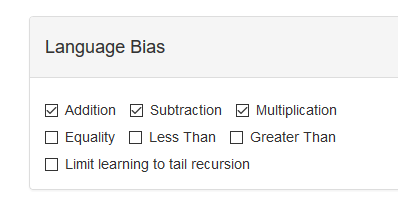
\includegraphics[width=0.5\textwidth]{C5/bias_restriction.png}
\caption{Bias Restriction}
\end{figure}

\subsection{Handling errors}

Sometimes, it may not be possible to learn a program from a set of examples. They may be contradictory, or the tool may not be robust enough. In this case, you have a few options open to you :

\begin{itemize}
\item Try to remove certain examples to find out which one might be causing a contradiction.
\item Separate your function into multiple smaller ones. For example, a Merge Sort program could be separated into smaller splitting and comparision programs.
\end{itemize}

\pagebreak

\section{The Design Process}
Designing the user interface was not an easy process. While I knew the basic features of my UI, to be an iterative learning tool which takes examples as input and displays a learned Haskell program as output, I did not have much of an idea of how to display this to the user. I chose to represent the input fields as a table or spreadsheet as it seemed like an interface that is commonly known and easy to understand. The concept of adding rows and columns, and having functions that work over those columns is one common to spreadsheet tools like Excel, and I thought this would help illustrate the concept of my tool to new users unfamiliar with IFP. \\ \\
One UI approach I considered was writing the tool as a plugin for an existing spreadsheet program such as Excel or LibreOffice Calc. While this would have saved a majority of the frontend design and implementation work, it would have meant that my tool has to rely on user's knowledge of the host program, and limiting what features I could add. Instead, I decided to use an approach which was spreadsheet inspired but implemented in my own web-based UI.\\ \\
Now that I had chosen this approach, I had to design how it would look. Initially using paper sketches and online formatting tools, I started building a picture of what the UI would look like. However, my ideas started looking more like a table than a spreadsheet, as I would not need all the functionality a typical spreadsheet provides. In addition, Javascript libraries for making spreadsheets are quite hard to find and implement, while ones with table functionality are common, as tables are built-in HTML tag.

\section{Writing the Backend}
The first part of my tool that needed a backend was the part which generates skeleton rules. Instead of finding some way in ASP to enumerate over all possible rule bodies, it seemed easier to write a Java program to perform this generation. I chose Java as it is a language I am very familiar with, reducing the number of new technologies I would have to learn to start implementation. In addition, Java can be quite easy to maintain as the size of the project grows, although it can be overly verbose at times. \\ \\
After handling skeleton rule generation, the backend also needed to handle other tasks that could not be performed using ASP.
\begin{itemize}
\item Converting from ground \lstinline{choose} atoms as produced in the answer set to full choice rules. %{
\item Generating Haskell from the chosen ASP rules.
\item Running the Haskell program to auto-complete any examples.
\item Managing when to just run Haskell and when to re-learn.
\end{itemize} 
\mbox{} \\
While it might seem that converting from ASP to valid Haskell would be difficult, it turned out to be a surprisingly easy process due to the chosen subset of the target language and way I have defined rule bodies. Because there are only arithmetic operations with two arguments, the tool can use recursively iterate through the expression, building up the Haskell string as it runs using simple string formatting. It is equally easy to generate guard statements from the bodies of chosen \lstinline{match} rules %{

\section{Technologies Used}
To make use of the Java backend, I needed a UI framework which could easily integrate with it, while also not being too complicated to learn. In addition, I wanted a way to implement a web based UI instead of a traditional Desktop application, as it would allow the tool to be hosted on the cloud, available to anyone with a web browser.

\subsection{Play Framework and Akka}
Because I wanted to build a web app while having a Java backend, it made most sense to use the Play Framework \cite{Play} to link the two together. The Play Framework provides a way to easily integrate a HTML and Javascript frontend with a Java backend, through HTTP requests. Methods on the backend that need to be accessed on the frontend can be written into a Controller class, whose methods become exposed as \lstinline{GET}, \lstinline{POST} and \lstinline{DELETE} endpoints. These endpoints are then accessable in the frontend, through ajax calls written in the Javascript. \\ \\%{
Play also allows for processes to be ran in the background, asynchronously. This was useful for the tool, as I did not want it to be unresponsive while waiting for the potentially long time the learning task takes. To achieve this, I made use of Akka actors \cite{Akka}. Akka is a toolkit used to build concurrent systems made up from actors, abstract concurrent processes. As part of my backend, I define the learning task as one of these actors, which is initiated when the frontend submits a new task. Then, the frontend repeatedly queries the backend until the learning is complete, at which point the learned Haskell is returned.

\subsection{Bootstrap}
For the user interface, I wanted a quick, simple way to design it, looking clean and structured without anything overly complicated. To achieve this, I used Bootstrap \cite{Bootstrap}, a simple css and javascript library, containing a large built in collection of common HTML elements such as toolbars, modals, tables and tab. Having used Bootstrap in projects before, it was familiar enough that it made writing my initial UI frontend quick and painless, and allowed me to easily make changes based on user feedback.

\section{User Feedback and Evaluation}
To help with the design of the user interface, it was important to get feedback from users wherever possible. This feedback started with friends and supervisors, and was given informally as we discussed each stage of the UI. With friends, we frequently worked together and at such an early stage it is easy to ask for feedback and iterate based on this. \\ \\
As the UI came nearer to completion, I realised that more formal feedback was necessary. By getting in touch with younger students and family with a non-technical background, I could get more unbiased and descriptive feedback from a variety of perspectives. This feedback helped fix bugs, add extra features, gain new examples and uncover limitations in the learning.


\pagebreak
%\renewcommand\bibname{{References}}
%\bibliography{References}
%\bibliographystyle{plain}